\documentclass{article}

\usepackage{tikz}
\usetikzlibrary{positioning}


\begin{document}
% STYLES
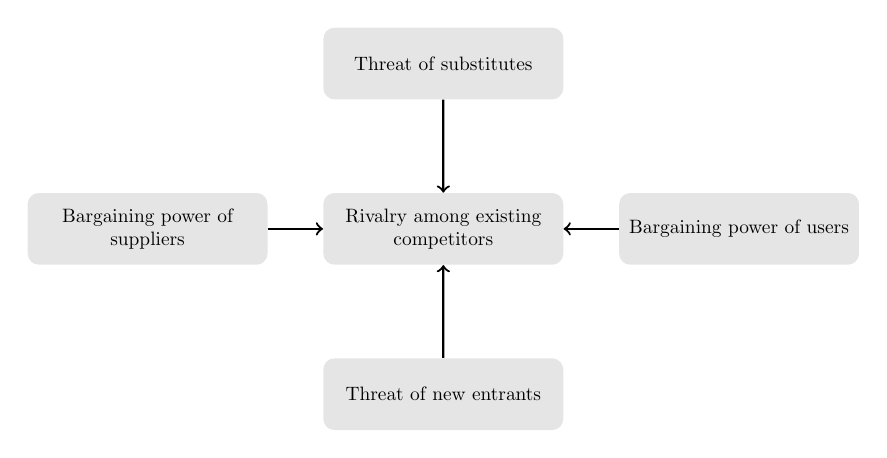
\begin{tikzpicture}[scale=0.7, transform shape]
% STYLES
\tikzset{%
    force/.style={%
node distance = 1cm, 
auto,
rectangle,
rounded corners, 
fill=black!10,
node distance=3cm,
inner sep=5pt, 
text width=4cm, 
text badly centered, 
minimum height=1.3cm
                          }
             }

% Draw forces
\node [force] (rivalry) {Rivalry among existing competitors};
\node [force, above of=rivalry] (substitutes) {Threat of substitutes};
\node [force, left=1cm of rivalry] (suppliers) {Bargaining power of suppliers};
\node [force, right=1cm of rivalry] (users) {Bargaining power of users};
\node [force, below of=rivalry] (entrants) {Threat of new entrants};
% Draw the links between forces
\path[->,thick] 
(substitutes) edge (rivalry)
(suppliers) edge (rivalry)
(users) edge (rivalry)
(entrants) edge (rivalry);
\end{tikzpicture} 
%\caption{Five Forces Diagram source:~%\cite{Porter:1980}}%
\end{document}